\documentclass[10pt,twocolumn,letterpaper]{article}

\usepackage{cvpr}
\usepackage{times}
\usepackage{epsfig}
\usepackage{graphicx}
\usepackage{amsmath}
\usepackage{amssymb}
\usepackage{gensymb}

% Include other packages here, before hyperref.

% If you comment hyperref and then uncomment it, you should delete
% egpaper.aux before re-running latex.  (Or just hit 'q' on the first latex
% run, let it finish, and you should be clear).
\usepackage[breaklinks=true,bookmarks=false]{hyperref}

\cvprfinalcopy % *** Uncomment this line for the final submission

\def\cvprPaperID{****} % *** Enter the CVPR Paper ID here
\def\httilde{\mbox{\tt\raisebox{-.5ex}{\symbol{126}}}}

% Pages are numbered in submission mode, and unnumbered in camera-ready
%\ifcvprfinal\pagestyle{empty}\fi
\setcounter{page}{1}
\begin{document}

%%%%%%%%% TITLE
\title{\LaTeX\ Detecting Hand Direction for Computer Interaction}

\author{Ben Mattinson and David Gaddy\\
Massachusetts Institute of Technology\\
77 Massachusetts Ave. Cambridge, MA 02139\\
{\tt\small bmatt@mit.edu, dgaddy@mit.edu}
% For a paper whose authors are all at the same institution,
% omit the following lines up until the closing ``}''.
% Additional authors and addresses can be added with ``\and'',
% just like the second author.
% To save space, use either the email address or home page, not both
}

\maketitle
%\thispagestyle{empty}

%%%%%%%%% ABSTRACT
\begin{abstract}
We present a method for detecting the direction of a pointing hand in an image for the purpose of creating a computer interface based on pointing.  Given an image that is dominated by a pointing hand, we use regression to determine where it points.  We collected a set of images to use for comparing performace on this task.  We evaluated the performance of two different features for the regression: convolutional neural networks and histograms of oriented gradients.  We also compared two different methods of performing the regression: K-nearest neighbors and least squares linear regression.  This work differs from many previous works in that it focuses on detecting the angle of a single finger in relation to the screen rather than on estimating hand poses or recognizing gestures.

\end{abstract}

%%%%%%%%% BODY TEXT
\section{Introduction}

Gesture recognition is an important problem for Human Computer Interaction because hands provide a very natural way to interact with the computer. Users are used to using their hands to manipulate the world and often use their hands when communicating ideas to other people. Giving computers the ability to recognize gestures would allow people to manipulate objects on a computer in a way that mimics the way they manipulate the world and communicate with others, instead of forcing them to use an artificial form of manipulation like a computer mouse. There are also other related applications for this technology, such as the interpretation of sign language.

The task of gesture recognition is often divided into two parts: first detecting hands in an image, and second recognizing the gesture a hand is making. Detecting the hands deals with finding local patches of pixels where a hand appears in an image. In order to do this, the computer must be able to differentiate hands from other objects in the background and from other parts of the body. Recognizing hands differs from many object recognition tasks, such as face detection, because the hands have many degrees of freedom that allow them to appear very different in images based on the gesture being made. For this reason, hand detection is often done by modeling skin color, but it has also been done by classifying shapes and combinations of the two methods.

Hand gesture recognition deals with the problem of, given a patch of pixels that represents a hand, determining the configuration the hand is in. One approach to this problem is modeling the joints of the hand and using image data to determine the position of each joint, but because of the complexity of this model, an example based approach is often used instead. In the example based approach, hand images are compared against examples using various features to find an example with a similar hand configuration. This approach is similar to the problem of object classification since different configurations of a hand look like different objects when projected onto a two dimensional image.

%-------------------------------------------------------------------------
\section{Previous work}

\subsection{Hand detection in images}

Because the shape of hands varies greatly based on the position and configuration of a hand, color is often used as a primary feature for detecting hands in images. In \cite{van2009haarlet}, Bergh et al. modeled skin colors with a Gaussian Mixture Model of skin color and combined this with a color histogram of faces found with a face detector. By combining both the general skin color model with a scene specific skin color, they were able to detect skin accurately. To distinguish hands from other skin, they took the largest connected regions of skin that were not the face (determined using the face detector). Their method was reported to be more robust to lighting and different users than more basic color models, though they still encountered problems when faces and hands overlapped in images.

Other methods for detecting hands involve looking at shape. Ong and Bowden \cite{ong2004boosted} trained a tree of boosted classifiers to find hands in images. To deal with the many different possible shapes of the hands, the first level of the tree proposed possible hand locations that were then put through classifiers lower in the tree that were trained to detect specific hand configurations. They reported a 99.8\% success rate on hand detection.

One last cue used for detecting hands is depth information. To deal with the problems of detecting hands with color alone (namely overlapping skin regions), Bergh and Gool used depth images taken with an infrared depth camera in addition to color in \cite{van2011combining}. By placing the restriction that the hands be held a certain threshold in front of the face (determined using a combination of a face detector and depth image) they were able to accurately detect hand regions, even when they overlapped with other skin.

\subsection{Hand gesture recognition}

One approach to recognizing hand gestures is to build a model of the joints of the hand and to try to determine the location of these points on an image. Erol et al. give a survey of such techniques in \cite{erol2007vision}. The full kinematic model of a hand has 27 degrees of freedom. To deal with all of these degrees of freedom, constraints of the ranges of motion for each joint and joint angle dependencies are considered. In addition, methods such as placing markers on the hands or tracking the movement of hands through time have been used to make detecting the joint locations possible.

Another approach involves comparing the hand image to a set of example images for different gestures. This approach builds a classifier that attempts to put a given image into a class that represents the type of gesture being made. To do this, a vector of features is extracted from the image and compared against the features on the given examples. A variety of features and classifier types have been used to do this.

One approach, used by Freeman and Roth \cite{freeman1995orientation}, used a histogram of gradient orientations in the image as a feature vector. Using gradients made these features invariant to lighting and using a histogram made it invariant to translation. By finding the training feature vector that is most similar to the vector for a given image, they were able to distinguish between 10 different hand gestures.

More recently, neural networks have been employed for accurate continuous hand pose estimation. Tompson et al. \cite{tompson2014real} used a deep convolutional neural network to identify the positions of key points on hands in RGB+Depth images. They trained the neural network to recognize certain hand features and used the results to infer the hand pose.

\subsection{Finger detection and gesture recognition}

Several different methods of detecting fingers in images exist. Most involve first detecting a hand in the image and using information about the hand position and components to identify fingers. Hands can be detected using some of the aforementioned techniques, e.g. color or shape. Lee and Lee \cite{lee2011vision} used color and information about consecutive motion between frames of video for hand detection. After isolating the hand from the image, they examined the curvature of the hand region for sharp curves to identify fingertips. To measure the direction of each fingertip, Lee and Lee selected two points along the edge of the finger, one on each side a set distance from the fingertip. They then measured the direction of the vector between the average of these two points and the fingertip.

\section{Methods}

\subsection{Problem setting} % may want to rename this

For this work, we decided to focus on the problem of finding the orientation of a hand given a region where the hand is known to be instead of detecting the hand in a larger image.  To do this, we made several assumptions about the images we processed.

First, we assume that the images have a clear background.  Although this assumption will often be broken in the target application of computer interaction, additional preprocessing could be done in a complete system to segment out the background of an image.  Methods for hand detection such as those described in the previous work section that use hand color, depth, or other cues could be used for this purpose.

Second, we assume that the hand is roughly at a constant distance from the camera and at roughly the same location in the image.  For the application of pointing at a computer screen, this assumption is fairly reasonable since a user's distance to the screen will usually vary by only a few feet at most and is likely to hold their hand directly in front of the screen to point at it.  To make the system more robust or for other applications, the location of the hand in an image could be detected using the methods described in previous work and our system could be passed only the region around a detected image.  Additionally, we could make our system more robust to distance and location by training on images that contained hands at different distances and locations.

\subsection{Data collection and evaluation}

We collected a set of images to evaluate the relative effectiveness of different methods.  These images were collected from a standard webcam directly above a computer screen.  Each picture contained a pointing hand to recognize on a blank background.  The hand was approximately one foot away from the camera and screen.  To keep hand location consistent, the user was shown a video of their hand as they recorded and attempted to keep their hand on a crosshair overlayed at the center of the image.  A dot was displayed on the screen and the user pointed at the dot as it moved across the screen.  The dot moved along a seven by seven grid with spacing of 80 pixels and for each location a picture was taken of the user pointing at that location from the webcam.  We repeated this grid collection procedure 15 times, collecting a total of 735 images.

For evaluation, we used 15-fold cross validation, except the groups were chosen based on the grid collection iteration instead of a random sample.  For each data group, we trained on the other 14 groups and evaluated performance on the group, then we took the average performance for all 15 groups.  The reason for choosing groups based on collection iteration instead of random sampling is that images collected during the same scanning process tended to be more similar so training with images in the same iteration as the test data artificially increased scores.

It is important to note that the data collected has inherent noise because people are limited in precision for pointing at a location on a screen.  The location a user thinks they are pointing at may depend on the relative orientations of their eyes, their hands, and the screen.  For this reason, no system will be able to achieve perfect results.

\subsection{Overview of methods}

Created feature vectors to describe image.  We evaluated two different methods of extracting these feature vectors: convolutional neural networks and histograms of gradient orientations.  We then trained regressors from these features to the ground truth location.  We experimented with several different types of regressors and report here the results for least squares linear regression and K-nearest neighbors regression.  Other regression methods did not provide any significant improvement.  We used the scikit-learn library implementation of these methods \cite{scikit-learn}.

\subsection{Convolutional neural networks}

One source of features we evaluated was convolutional neural networks.  Convolutional neural networks have been used to get state of the art results in object recognition tasks such as the ILSVRC-2012 competition \cite{krizhevsky2012imagenet}.  It has been found that the values of neurons in the upper layers of the network provide good features for computer vision tasks, even though the network was not trained for these tasks \cite{donahue2013decaf}.  For our features, we used the neural network model trained by fdjslf People for fjksdlfj task.  \cite{jia2014caffe}  We ran their model and extracted the outputs of the final fully connected layer before the softmax layer that 

\begin{figure*}
	\begin{center}
		%\fbox{\rule{0pt}{2in} \rule{.9\linewidth}{0pt}}
		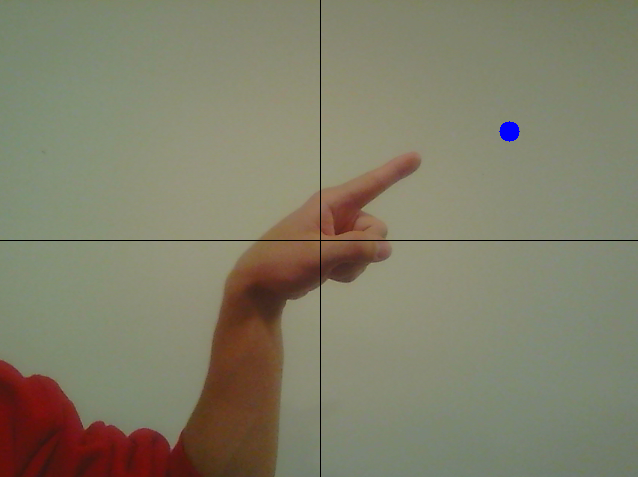
\includegraphics[height=140px]{figures/PointImage.png}
		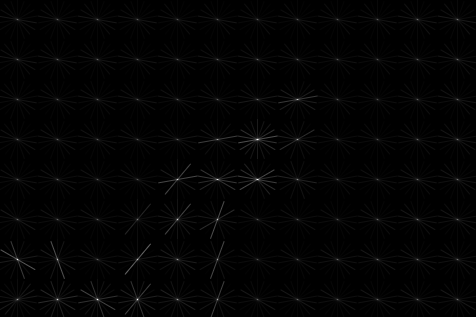
\includegraphics[height=140px]{figures/PointHOG.png}
	\end{center}
	\caption{An image (on the left) and our corresponding HOG output (on the right). The location calculated by our algorithm is illustrated by the blue dot on the left image.}
	\label{fig:pointImages}
\end{figure*}

\subsection{Histogram of Gradients}

We also evaluated the Histogram of Oriented Gradients (HOG) feature descriptor \cite{dalal2005histograms} as a means to detect the location and orientation of the pointing hand. This expands on work done by Freeman and Roth, who used gradients to detect hand gestures. We used a variant of the R-HOG algorithm described by Dalal and Triggs in \cite{dalal2005histograms}. We divided the image into an 8 $\times$ 12 grid, yielding approximately 53 $\times$ 60 pixel cells. We divided orientations into 9 bins from $0\degree$-$360\degree$. In contrast to the block-normalization scheme used by Dalal and Triggs, all cells were scaled by the same value so the $l^2$ norm of the cells was 1.

\subsection{Classifier}
We experimented with several different classifiers including k-Nearest Neighbors, linear regression, and SVM. We found that a combination of k-nearest neighbors and linear regression worked best across a wide variety of data. We trained the k-nearest neighbors and linear regression models from sci-kit learn separately on 15 sets of test data comprised of the HOG features computed from each image. These models each predicted a location based on HOG input. These locations were averaged together and fed into a smoothing algorithm to compute the final location.

\subsection{Smoothing}
In order to make the system more robust to noise, we both smooth the location and eliminate outliers. Let $x[n]$ be the location at frame $n$ and $u[n]$ be the location output from the k-NN and linear regression combination at frame $n$. Outliers are eliminated if
\begin{equation}
	\sqrt{\sum_{i=n-l}^{n}(u[n]-x[i])^2} >= \epsilon
\end{equation}
where $l$ and $\epsilon$ are parameters representing the amount of history to remember for computing outliers and the sensitivity to outliers, respectively. We used $l=10$ and $\epsilon=200$. Smoothing is implemented by the formula 
\begin{equation}
	x[n+1] = \left\{
		\begin{array}{l l}
			\lambda x[n] + (1-\lambda)u[n] & \qquad \text{if not an outlier} \\
			x[n] & \qquad \text{otherwise}
		\end{array}
	\right.
\end{equation}
 where $\lambda$ is a smoothing parameter between 0 and 1. We used $\lambda=0.5$ to balance quick responsiveness with robustness to noise.

\section{Results}

\subsection{Performance on test data}

\subsubsection{Performance of Different Classifiers}
We evaluated the performance of both convolution neural networks and HOG with k-Nearest Neighbors and Linear Regression. The results from our tests our given in figure \ref{fig:hist}, which is a histogram of the error of the different classifiers. The error is the euclidean distance measured in pixels between the predicted point and the actual point.
\begin{figure*}
	\begin{center}
		%\fbox{\rule{0pt}{2in} \rule{.9\linewidth}{0pt}}
		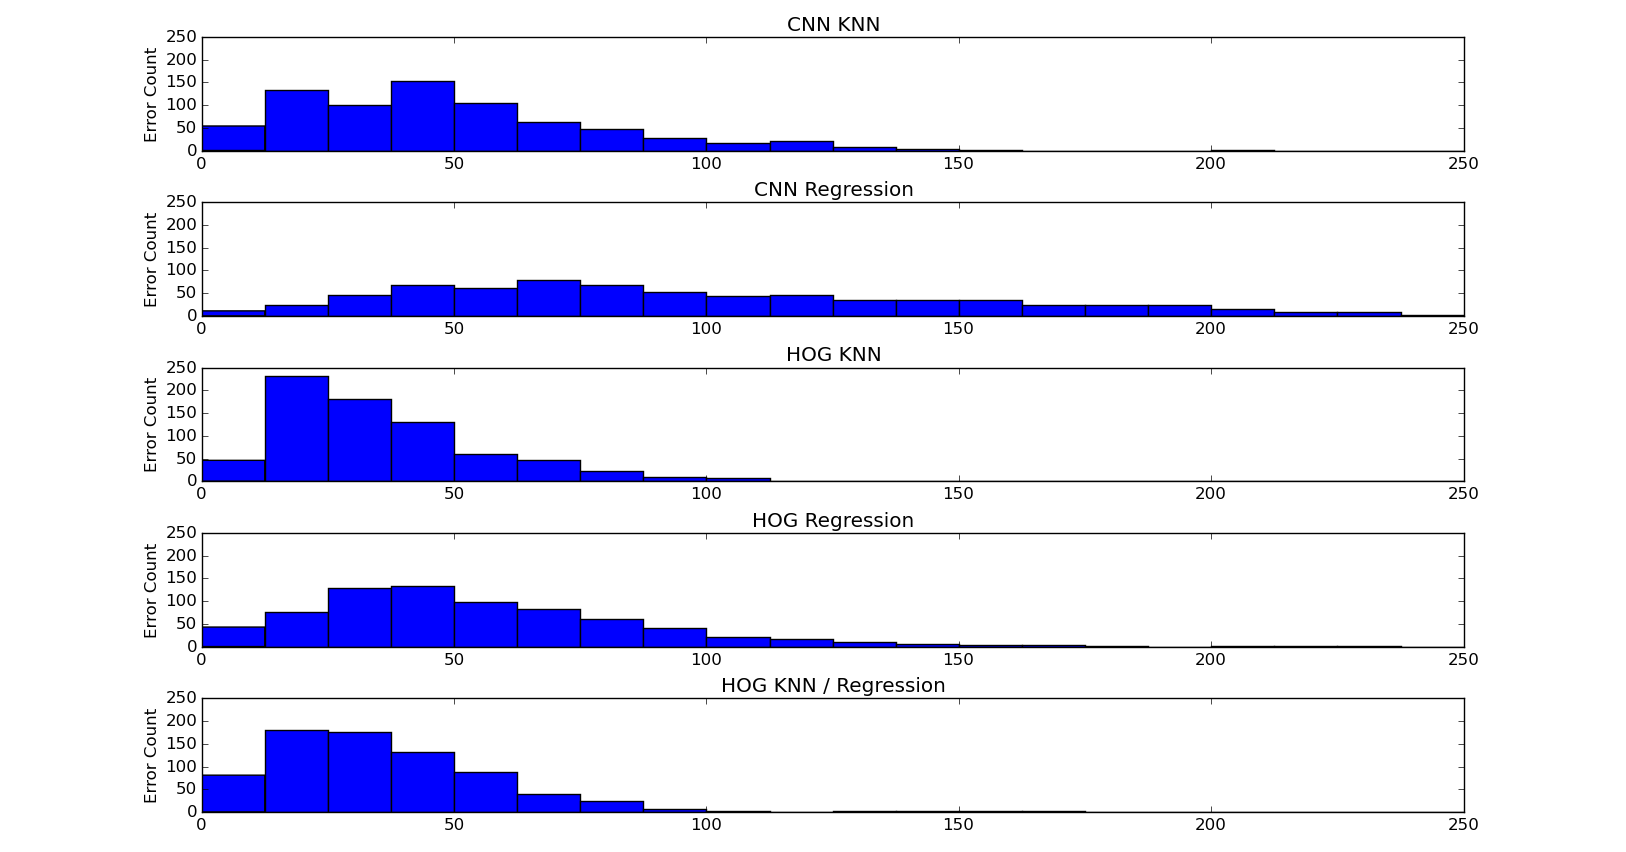
\includegraphics[width=0.9\linewidth]{figures/ClassifierErrorHist.png}
	\end{center}
	\caption{An image (on the left) and our corresponding HOG output (on the right). The location calculated by our algorithm is illustrated by the blue dot on the left image.}
	\label{fig:hist}
\end{figure*}
\subsection{Evaluation as a Computer Interaction Device}

To test our system's effectiveness for computer interaction, we used the HOG feature based system to predict where a user was pointing at a computer screen.  We used the prediction to move a dot on the screen, which simulated the movement of a computer mouse.  Something about effectiveness fdjslfj

The time to process an image using convolutional neural networks was too high to allow for real time computer interaction, since each frame took several seconds to process.  Using a GPU to process frames would greatly increase the speed and should allow for the possibility of using these features in a real time system.

\section{Conclusion}

%-------------------------------------------------------------------------

{\small
\bibliographystyle{ieee}
\bibliography{paper}
}

\end{document}
